\documentclass[10pt]{article}
\usepackage[a4paper,landscape,margin=1.3cm,top=1.5cm,bottom=1.4cm]{geometry}
\usepackage[T1]{fontenc}
\usepackage{newtxtext,newtxmath}
\usepackage[scaled=0.86]{beramono}
\usepackage{tikz}
\usetikzlibrary{positioning,arrows.meta,fit,backgrounds,calc,shapes.geometric,shapes.misc}
\usepackage{xcolor}
\usepackage{fancyhdr}
\usepackage{enumitem}
\usepackage[hidelinks]{hyperref}
\setlist{itemsep=1pt,topsep=2pt,leftmargin=1.2em}

\definecolor{ablue}{HTML}{1D4E89}
\definecolor{aorange}{HTML}{C2410C}
\definecolor{agreen}{HTML}{3E7B32}
\definecolor{apurple}{HTML}{6B4C9A}
\definecolor{agrey}{HTML}{52606D}
\definecolor{fdata}{HTML}{EAF1F8}
\definecolor{fmodel}{HTML}{E8EEF9}
\definecolor{fnew}{HTML}{FDEDE3}
\definecolor{feval}{HTML}{EAF5E6}
\definecolor{faudit}{HTML}{F1ECF8}
\definecolor{fgrey}{HTML}{F3F5F8}

\pagestyle{fancy}\fancyhf{}
\fancyhead[L]{\small\color{gray}Alma Models: Architecture}
\fancyhead[R]{\small\color{gray}As implemented in the repository at commit 43b463b}
\fancyfoot[C]{\small\thepage}
\renewcommand{\headrulewidth}{0.3pt}

\tikzset{
  >={Stealth[length=2.4mm]},
  box/.style={draw=#1!70!black,fill=#1!8,rounded corners=2pt,align=center,font=\small,inner sep=3.5pt,minimum height=8mm,line width=0.5pt},
  box/.default=ablue,
  data/.style={box=ablue,fill=fdata},
  model/.style={box=ablue,fill=fmodel},
  newb/.style={box=aorange,fill=fnew,line width=0.8pt},
  evalb/.style={box=agreen,fill=feval},
  audb/.style={box=apurple,fill=faudit},
  greyb/.style={box=agrey,fill=fgrey},
  op/.style={circle,draw=agrey,fill=white,inner sep=1pt,font=\footnotesize,minimum size=6mm},
  arr/.style={->,line width=0.6pt,draw=agrey},
  darr/.style={->,line width=0.6pt,draw=agrey,dashed},
  rarr/.style={->,line width=1.1pt,draw=ablue},
  lab/.style={font=\footnotesize\itshape,text=agrey,align=center},
  group/.style={draw=#1!60,dashed,rounded corners=4pt,inner sep=6pt,line width=0.5pt},
  gtitle/.style={font=\scriptsize\bfseries,text=#1,anchor=south west,inner sep=1pt},
}
\newcommand{\pagetitle}[2]{{\noindent\Large\bfseries\color{ablue}#1}\par\vspace{1pt}{\noindent\small\color{agrey}#2}\par\vspace{6pt}}
\newcommand{\keyline}{\par\vspace{4pt}\noindent{\scriptsize
\tikz\node[data,minimum height=3mm,minimum width=5mm,inner sep=1.5pt]{};\ data\quad
\tikz\node[model,minimum height=3mm,minimum width=5mm,inner sep=1.5pt]{};\ original Alma model\quad
\tikz\node[newb,minimum height=3mm,minimum width=5mm,inner sep=1.5pt]{};\ added by the 1 Nov 2026 audit\quad
\tikz\node[evalb,minimum height=3mm,minimum width=5mm,inner sep=1.5pt]{};\ evaluation\quad
\tikz\node[audb,minimum height=3mm,minimum width=5mm,inner sep=1.5pt]{};\ audit\quad
\tikz\node[greyb,minimum height=3mm,minimum width=5mm,inner sep=1.5pt]{};\ baseline / other\quad
\tikz\draw[rarr](0,0)--(0.6,0);\ latent rollout (carried state)\quad
\tikz\draw[darr](0,0)--(0.6,0);\ used in training only / optional}}

\begin{document}

% =====================================================================================================================
% PAGE 1  End-to-end system
% =====================================================================================================================
\pagetitle{1. End-to-end system architecture}{The pipeline every market project followed (oil, power, gas, crypto), with the audit and forward-test layers added on 1 November 2026. Source: \texttt{tools/<project>/}, \texttt{runs/<project>/}, \texttt{docs/*\_prereg.md}, \texttt{tools/forward/}.}

\begin{center}
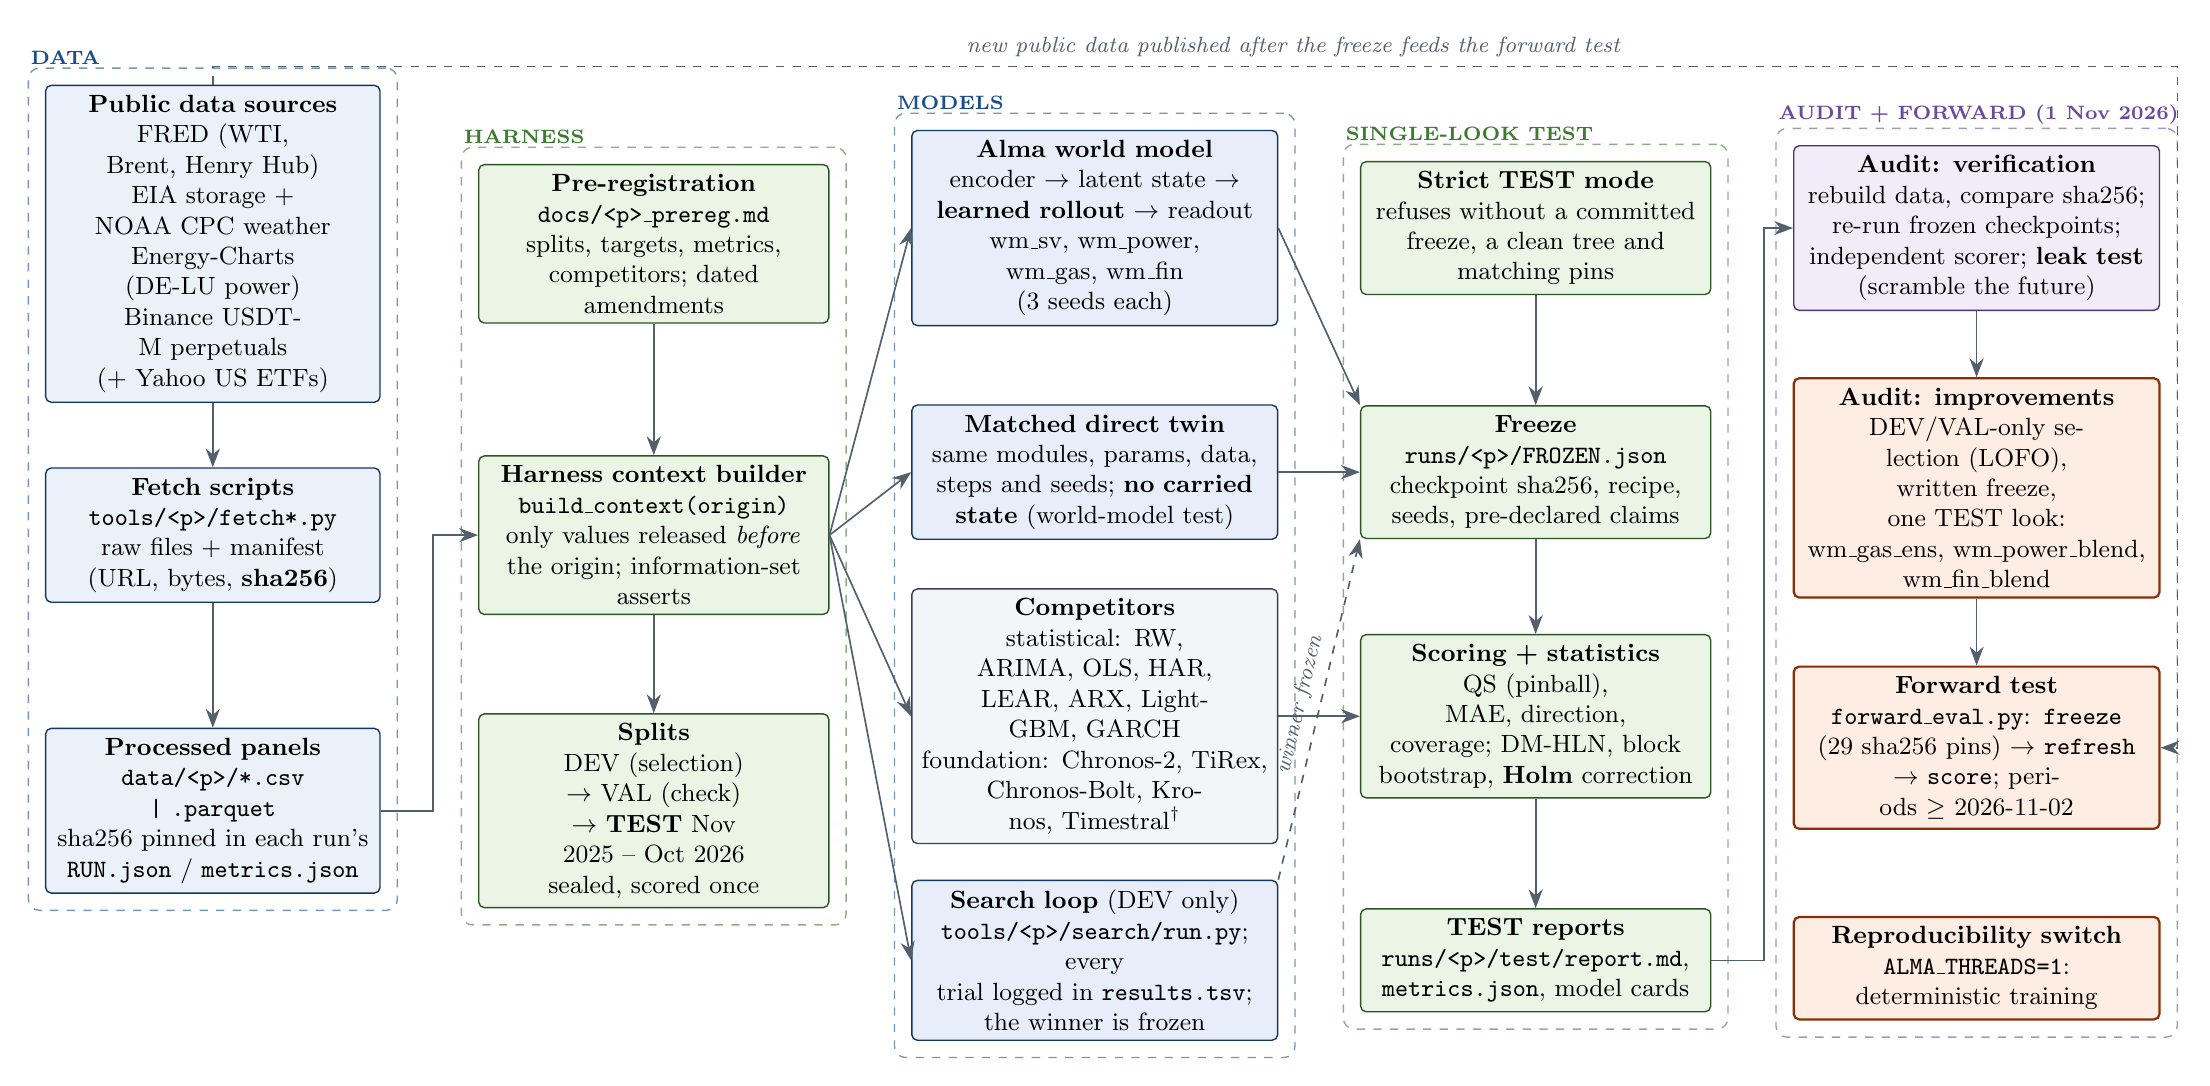
\begin{tikzpicture}[x=1cm,y=1cm]
% DATA
\node[data,text width=4.0cm] (src) at (2.3,0.3) {\textbf{Public data sources}\\FRED (WTI, Brent, Henry Hub)\\EIA storage + NOAA CPC weather\\Energy-Charts (DE-LU power)\\Binance USDT-M perpetuals\\(+ Yahoo US ETFs)};
\node[data,text width=4.0cm] (fetch) at (2.3,-3.4) {\textbf{Fetch scripts}\\\texttt{tools/<p>/fetch*.py}\\raw files + manifest\\(URL, bytes, \textbf{sha256})};
\node[data,text width=4.0cm] (proc) at (2.3,-6.9) {\textbf{Processed panels}\\\texttt{data/<p>/*.csv | .parquet}\\sha256 pinned in each run's\\\texttt{RUN.json} / \texttt{metrics.json}};
\draw[arr] (src)--(fetch); \draw[arr] (fetch)--(proc);
% HARNESS
\node[evalb,text width=4.2cm] (prereg) at (7.9,0.3) {\textbf{Pre-registration}\\\texttt{docs/<p>\_prereg.md}\\splits, targets, metrics,\\competitors; dated amendments};
\node[evalb,text width=4.2cm] (ctx) at (7.9,-3.4) {\textbf{Harness context builder}\\\texttt{build\_context(origin)}\\only values released \emph{before}\\the origin; information-set\\asserts};
\node[evalb,text width=4.2cm] (splits) at (7.9,-6.9) {\textbf{Splits}\\DEV (selection) $\to$ VAL (check)\\$\to$ \textbf{TEST} Nov 2025 -- Oct 2026\\sealed, scored once};
\draw[arr] (proc.east) -- (5.1,-6.9) |- (ctx.west);
\draw[arr] (prereg)--(ctx); \draw[arr] (ctx)--(splits);
% MODELS
\node[model,text width=4.4cm] (wm) at (13.5,0.5) {\textbf{Alma world model}\\encoder $\to$ latent state $\to$\\\textbf{learned rollout} $\to$ readout\\wm\_sv, wm\_power, wm\_gas, wm\_fin\\(3 seeds each)};
\node[model,text width=4.4cm] (twin) at (13.5,-2.6) {\textbf{Matched direct twin}\\same modules, params, data,\\steps and seeds; \textbf{no carried}\\\textbf{state} (world-model test)};
\node[greyb,text width=4.4cm] (base) at (13.5,-5.7) {\textbf{Competitors}\\statistical: RW, ARIMA, OLS, HAR,\\LEAR, ARX, LightGBM, GARCH\\foundation: Chronos-2, TiRex,\\Chronos-Bolt, Kronos, Timestral$^{\dagger}$};
\node[model,text width=4.4cm] (search) at (13.5,-8.8) {\textbf{Search loop} (DEV only)\\\texttt{tools/<p>/search/run.py}; every\\trial logged in \texttt{results.tsv};\\the winner is frozen};
\draw[arr] (ctx.east) -- (wm.west); \draw[arr] (ctx.east) -- (twin.west); \draw[arr] (ctx.east) -- (base.west); \draw[arr] (ctx.east) -- (search.west);
% TEST
\node[evalb,text width=4.2cm] (strict) at (19.1,0.5) {\textbf{Strict TEST mode}\\refuses without a committed\\freeze, a clean tree and\\matching pins};
\node[evalb,text width=4.2cm] (freeze) at (19.1,-2.6) {\textbf{Freeze}\\\texttt{runs/<p>/FROZEN.json}\\checkpoint sha256, recipe,\\seeds, pre-declared claims};
\node[evalb,text width=4.2cm] (score) at (19.1,-5.7) {\textbf{Scoring + statistics}\\QS (pinball), MAE, direction,\\coverage; DM-HLN, block\\bootstrap, \textbf{Holm} correction};
\node[evalb,text width=4.2cm] (rep) at (19.1,-8.8) {\textbf{TEST reports}\\\texttt{runs/<p>/test/report.md},\\\texttt{metrics.json}, model cards};
\draw[arr] (wm.east)--(freeze.north west); \draw[arr] (twin.east)--(freeze.west); \draw[arr] (base.east)--(score.west);
\draw[darr] (search.north east) -- node[lab,above,sloped]{winner frozen} (freeze.south west);
\draw[arr] (strict)--(freeze); \draw[arr] (freeze)--(score); \draw[arr] (score)--(rep);
% AUDIT
\node[audb,text width=4.4cm] (aud) at (24.7,0.5) {\textbf{Audit: verification}\\rebuild data, compare sha256;\\re-run frozen checkpoints;\\independent scorer; \textbf{leak test}\\(scramble the future)};
\node[newb,text width=4.4cm] (imp) at (24.7,-2.8) {\textbf{Audit: improvements}\\DEV/VAL-only selection (LOFO),\\written freeze, one TEST look:\\wm\_gas\_ens, wm\_power\_blend,\\wm\_fin\_blend};
\node[newb,text width=4.4cm] (fwd) at (24.7,-6.1) {\textbf{Forward test}\\\texttt{forward\_eval.py}: \texttt{freeze}\\(29 sha256 pins) $\to$ \texttt{refresh}\\$\to$ \texttt{score}; periods $\geq$ 2026-11-02};
\node[newb,text width=4.4cm] (repro) at (24.7,-8.9) {\textbf{Reproducibility switch}\\\texttt{ALMA\_THREADS=1}:\\deterministic training};
\draw[arr] (rep.east) -- (22.0,-8.8) |- (aud.west);
\draw[arr] (aud)--(imp); \draw[arr] (imp)--(fwd);
\draw[darr] (src.north) -- (2.3,2.55) -- node[lab,above,pos=0.55]{new public data published after the freeze feeds the forward test} (27.25,2.55) |- (fwd.east);
\begin{scope}[on background layer]
\node[group=ablue,fit=(src)(proc)] (g1) {}; \node[gtitle=ablue] at (g1.north west) {DATA};
\node[group=agreen,fit=(prereg)(splits)] (g2) {}; \node[gtitle=agreen] at (g2.north west) {HARNESS};
\node[group=ablue,fit=(wm)(search)] (g3) {}; \node[gtitle=ablue] at (g3.north west) {MODELS};
\node[group=agreen,fit=(strict)(rep)] (g4) {}; \node[gtitle=agreen] at (g4.north west) {SINGLE-LOOK TEST};
\node[group=apurple,fit=(aud)(repro)] (g5) {}; \node[gtitle=apurple] at (g5.north west) {AUDIT + FORWARD (1 Nov 2026)};
\end{scope}
\end{tikzpicture}
\end{center}
{\scriptsize $^{\dagger}$Timestral-5M is scored but excluded from claims because its training data overlap the test period (flagged ``contaminated'' in every report).}
\keyline

% =====================================================================================================================
% PAGE 2  World model vs direct twin
% =====================================================================================================================
\newpage
\pagetitle{2. The core design: world model vs matched direct twin}{Every Alma model has a twin with identical modules, parameter count, data, training steps and seeds. Only how the latent state advances differs. This comparison is the project's mandatory ``world-model test'' (\texttt{alma\_goal.md} \S2).}

\begin{center}
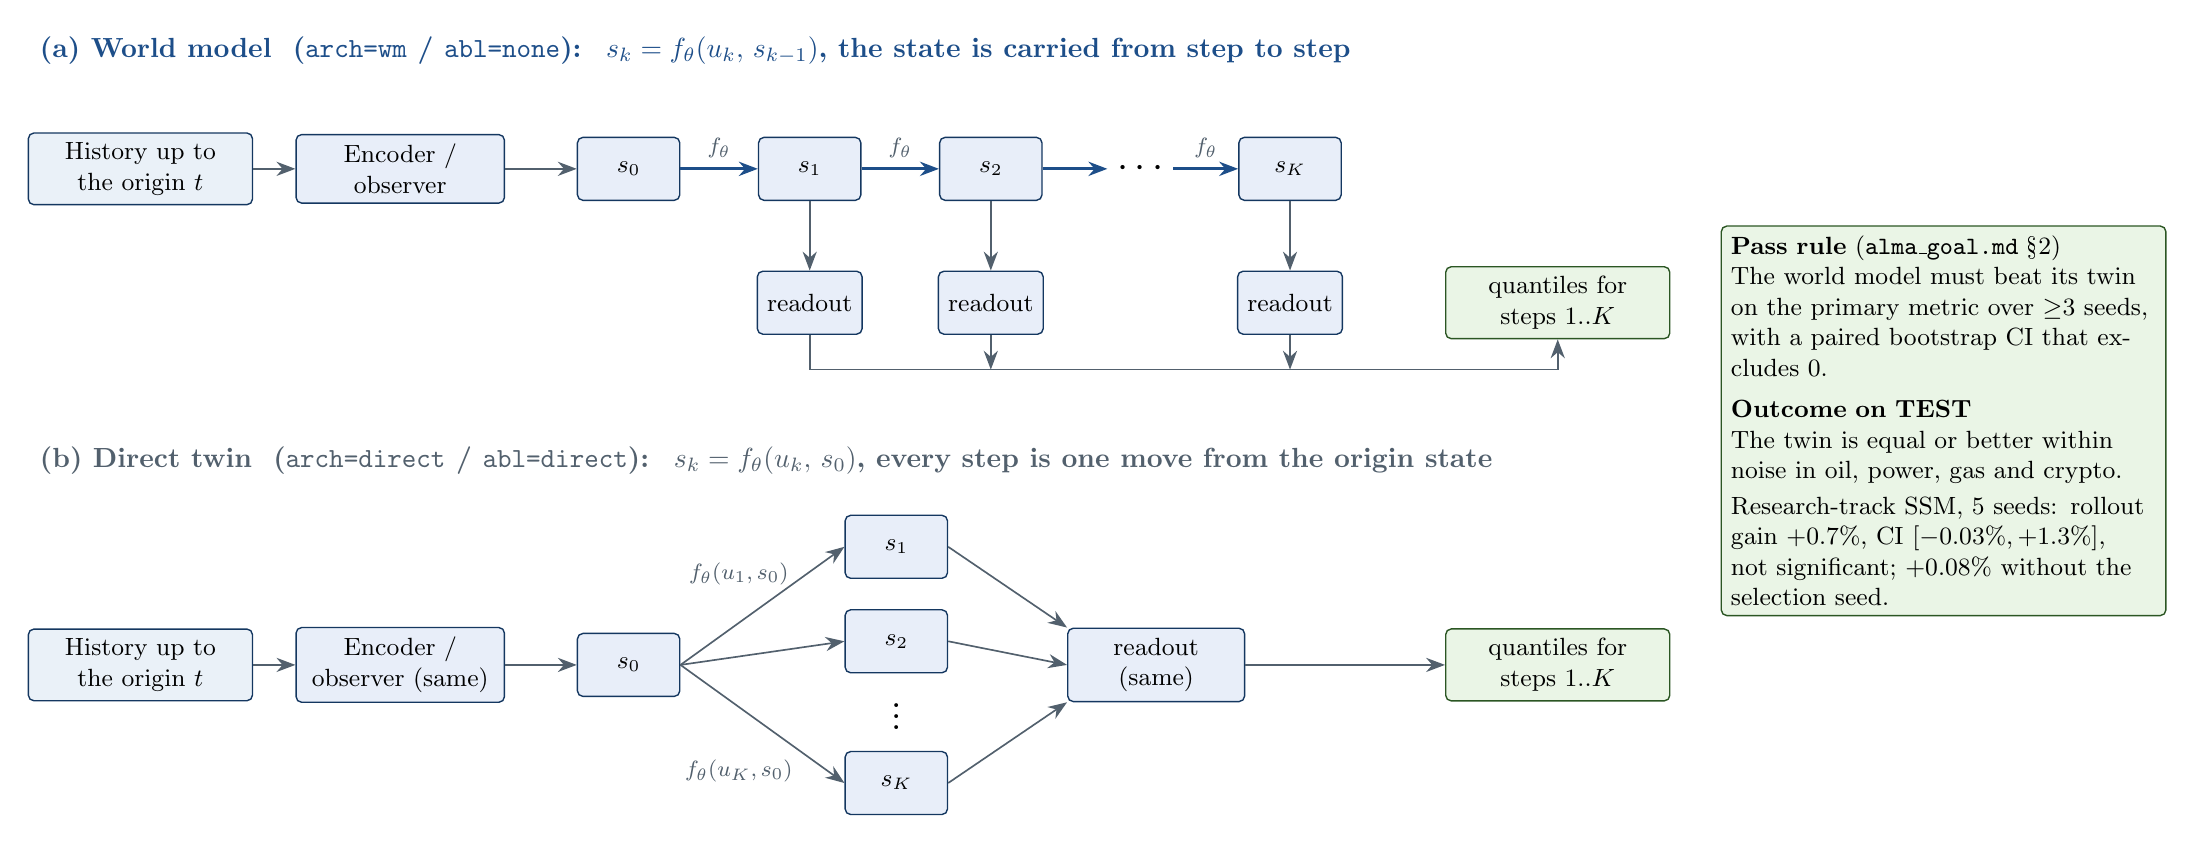
\begin{tikzpicture}[x=1cm,y=1cm]
\node[font=\normalsize\bfseries,text=ablue,anchor=west] at (0,1.5) {(a) World model \ (\texttt{arch=wm} / \texttt{abl=none}): \ $s_k = f_\theta(u_k,\,s_{k-1})$, the state is carried from step to step};
\node[data,text width=2.6cm] (h1) at (1.4,0) {History up to\\the origin $t$};
\node[model,text width=2.4cm] (e1) at (4.7,0) {Encoder /\\observer};
\node[model,minimum width=1.3cm] (s0) at (7.6,0) {$s_0$};
\node[model,minimum width=1.3cm] (s1) at (9.9,0) {$s_1$};
\node[model,minimum width=1.3cm] (s2) at (12.2,0) {$s_2$};
\node[font=\Large] (sd) at (14.1,0) {$\cdots$};
\node[model,minimum width=1.3cm] (sk) at (16.0,0) {$s_K$};
\draw[arr] (h1)--(e1); \draw[arr] (e1)--(s0);
\draw[rarr] (s0)--node[lab,above]{$f_\theta$}(s1); \draw[rarr] (s1)--node[lab,above]{$f_\theta$}(s2);
\draw[rarr] (s2)--(sd); \draw[rarr] (sd)--node[lab,above]{$f_\theta$}(sk);
\node[model] (r1) at (9.9,-1.7) {readout}; \node[model] (r2) at (12.2,-1.7) {readout}; \node[model] (rk) at (16.0,-1.7) {readout};
\draw[arr] (s1)--(r1); \draw[arr] (s2)--(r2); \draw[arr] (sk)--(rk);
\node[evalb,text width=2.6cm] (q1) at (19.4,-1.7) {quantiles for\\steps $1..K$};
\draw[arr] (r1.south) -- (9.9,-2.55) -- (19.4,-2.55) -- (q1.south);
\draw[arr] (r2.south) -- (12.2,-2.55); \draw[arr] (rk.south) -- (16.0,-2.55);
% twin
\node[font=\normalsize\bfseries,text=agrey,anchor=west] at (0,-3.7) {(b) Direct twin \ (\texttt{arch=direct} / \texttt{abl=direct}): \ $s_k = f_\theta(u_k,\,s_0)$, every step is one move from the origin state};
\node[data,text width=2.6cm] (h2) at (1.4,-6.3) {History up to\\the origin $t$};
\node[model,text width=2.4cm] (e2) at (4.7,-6.3) {Encoder /\\observer (same)};
\node[model,minimum width=1.3cm] (t0) at (7.6,-6.3) {$s_0$};
\node[model,minimum width=1.3cm] (t1) at (11.0,-4.8) {$s_1$};
\node[model,minimum width=1.3cm] (t2) at (11.0,-6.0) {$s_2$};
\node[font=\Large] at (11.0,-6.85) {$\vdots$};
\node[model,minimum width=1.3cm] (tk) at (11.0,-7.8) {$s_K$};
\draw[arr] (h2)--(e2); \draw[arr] (e2)--(t0);
\draw[arr] (t0.east)--(t1.west); \draw[arr] (t0.east)--(t2.west); \draw[arr] (t0.east)--(tk.west);
\node[lab] at (9.0,-5.15) {$f_\theta(u_1,s_0)$}; \node[lab] at (9.0,-7.65) {$f_\theta(u_K,s_0)$};
\node[model,text width=2.0cm] (tr) at (14.3,-6.3) {readout\\(same)};
\draw[arr] (t1.east)--(tr.north west); \draw[arr] (t2.east)--(tr.west); \draw[arr] (tk.east)--(tr.south west);
\node[evalb,text width=2.6cm] (q2) at (19.4,-6.3) {quantiles for\\steps $1..K$};
\draw[arr] (tr)--(q2);
% verdict
\node[evalb,text width=5.4cm,align=left] (ver) at (24.3,-3.2) {\textbf{Pass rule} (\texttt{alma\_goal.md} \S2)\\The world model must beat its twin on the primary metric over $\geq$3 seeds, with a paired bootstrap CI that excludes 0.\\[4pt]
\textbf{Outcome on TEST}\\The twin is equal or better within noise in oil, power, gas and crypto.\\[2pt]
Research-track SSM, 5 seeds: rollout gain $+0.7\%$, CI $[-0.03\%, +1.3\%]$, not significant; $+0.08\%$ without the selection seed.};
\end{tikzpicture}
\end{center}
\vspace{2mm}
{\small $u_k$ is the step-$k$ driver (calendar or phase clock, known or forecast exogenous inputs, lagged observations). Each project's twin is built by the same class with one flag changed: oil \texttt{SVWM(abl="direct")}, power \texttt{PhysWM(abl="direct")}, gas \texttt{GasNet(rollout=False)}, crypto \texttt{RSSM(abl="direct")}.}
\keyline

% =====================================================================================================================
% PAGE 3  wm_gas
% =====================================================================================================================
\newpage
\pagetitle{3. wm\_gas: storage-balance state-space world model (US natural-gas storage)}{\texttt{tools/gas/search/nets.py} (\texttt{GasNet}), wrapper \texttt{tools/gas/wm\_gas.py}. Frozen recipe: \texttt{arch=wm, assim=1, regime=1, d=32}, dropout 0.3, wd 0.05, 1,200 steps; seeds 0, 1, 2; trained on weeks released $\leq$ 2025-06-30.}

\begin{center}
\begin{tikzpicture}[x=1cm,y=1cm]
% drivers and bus
\node[data,text width=3.6cm] (u) at (2.0,4.3) {\textbf{Daily drivers} $u_d$ (14 days)\\week $W\!-\!1$: observed weather;\\week $W$: observed to the origin,\\then CPC forecast; normals, calendar};
\node[model,text width=2.5cm] (inp) at (5.8,4.3) {\textbf{Input MLP}\\Linear($d$) $\to$ GELU};
\draw[arr] (u)--(inp);
\draw[line width=0.6pt,draw=agrey] (inp.east) -- (19.9,4.3);
\node[lab,anchor=south] at (13.0,4.35) {each day: one step of the shared \texttt{GRUCell}($d$)};
\foreach \x in {9.9,11.4,12.9,16.9,18.4,19.9} \draw[arr] (\x,4.3) -- (\x,0.42);
% encoder
\node[data,text width=3.6cm] (g) at (2.0,0) {\textbf{Origin vector} $g$\\released weekly history, storage\\deficit, lagged weather anomalies,\\target-week calendar, HH price\\history, origin kind (Thu/Fri)};
\node[model,text width=2.5cm] (enc) at (5.8,0) {\textbf{Encoder}\\Linear(64) $\to$ GELU\\$\to$ Linear($d$) $\to$ tanh};
\node[model,minimum width=1.0cm] (z0) at (8.3,0) {$z_0$};
\draw[arr] (g)--(enc); \draw[arr] (enc)--(z0);
% week W-1
\node[model,minimum width=1.0cm] (a1) at (9.9,0) {$z_1$};
\node[model,minimum width=1.0cm] (a2) at (11.4,0) {$\cdots$};
\node[model,minimum width=1.0cm] (a7) at (12.9,0) {$z_7$};
\draw[rarr] (z0)--(a1); \draw[rarr] (a1)--(a2); \draw[rarr] (a2)--(a7);
\node[lab,fill=white,inner sep=1pt] at (11.4,1.25) {week $W\!-\!1$ (Sat--Fri): data assimilation};
% innovation
\node[model,text width=2.4cm] (flowp) at (12.2,-3.0) {model's regional\\flows $\Rightarrow \widehat{\Delta S}_{W-1}$};
\draw[arr] (a7.south) -- (a7.south|-flowp.north);
\node[op] (minus) at (14.6,-3.0) {$-$};
\node[data,text width=2.4cm] (rel) at (14.6,-4.9) {released $\Delta S_{W-1}$\\(EIA, per region)};
\draw[arr] (flowp)--(minus); \draw[arr] (rel)--(minus);
\node[model,text width=2.2cm] (inn) at (14.6,-1.5) {innovation\\Linear(5 $\to d$)};
\draw[arr] (minus)--(inn);
\node[op] (plus) at (14.6,0) {$+$};
\draw[rarr] (a7)--(plus); \draw[arr] (inn)--(plus);
% week W
\node[model,minimum width=1.0cm] (b1) at (16.9,0) {$z_8$};
\node[model,minimum width=1.0cm] (b2) at (18.4,0) {$\cdots$};
\node[model,minimum width=1.0cm] (b7) at (19.9,0) {$z_{14}$};
\draw[rarr] (plus)--(b1); \draw[rarr] (b1)--(b2); \draw[rarr] (b2)--(b7);
\node[lab,fill=white,inner sep=1pt] at (18.4,1.25) {target week $W$: imagination};
% readout
\node[model,text width=6.0cm,align=left,font=\footnotesize] (ro) at (19.9,-3.8) {\textbf{Monotone readout} (each day $d$, each of 5 regions $r$)\\[2pt]
$\begin{array}{@{}l@{}}\text{inj}_{rd} = \tfrac{a5_r}{7} + \tfrac{sd_r}{7}\big[\,\text{base}_r(z_d)\\
\qquad -\ \sum_b a^H_{rb}(z_d)\,\Delta\phi^H_b(\text{HDD}_d)\\
\qquad -\ \sum_b a^C_{rb}(z_d)\,\Delta\phi^C_b(\text{CDD}_d)\,\big]\end{array}$\\[3pt]
$a^H, a^C \geq 0$ (softplus); $\phi$ = monotone hinges, so demand rises with HDD and CDD; anchored at the 5-year average under normal weather.\\ \texttt{regime=1}: 3 regimes mixed by a softmax gate on $(z_d, u_d)$.};
\draw[arr] (b1.south) -- (b1.south|-ro.north); \draw[arr] (b7.south) -- (b7.south|-ro.north);
% outputs
\node[model,text width=3.0cm] (mb) at (25.3,0) {\textbf{Mass balance}\\$\Delta S_r = \sum_{d\in W}\text{inj}_{rd}$\\L48 $= \sum_{r=1}^{5}\Delta S_r$ (median)};
\draw[arr] (ro.east) -- (23.35,-3.8) |- (mb.west);
\node[model,text width=3.0cm] (cal) at (25.3,-2.7) {\textbf{Quantiles}\\median + holdout residual\\quantiles per origin kind\\(13 levels 0.025--0.975)};
\node[model,text width=3.0cm] (ens) at (25.3,-5.3) {\textbf{3-seed ensemble}\\quantile average, sorted\\$\to$ 6 series $\times$ 13 quantiles};
\draw[arr] (mb)--(cal); \draw[arr] (cal)--(ens);
\end{tikzpicture}
\end{center}
\vspace{-1mm}
\noindent{\small\textbf{Twin} (\texttt{wm\_gas\_direct}): each $z_d$ is one GRUCell step from $z_0$ (no state carried between days). The innovation is computed in the same way, so both models see identical inputs. Size: about 23.5K parameters per member. \textbf{TEST} (Thursday, 52 weeks): MAE 11.53\,Bcf, QS 4.59; the twin scores MAE 11.40, QS 4.57.}
\keyline

% =====================================================================================================================
% PAGE 4  wm_gas_ens
% =====================================================================================================================
\newpage
\pagetitle{4. wm\_gas\_ens: audit ensemble with OLS blend and adaptive intervals (new)}{\texttt{tools/gas/wm\_gas\_ens.py}; checkpoints in \texttt{winning\_models/gas\_wm\_gas\_ens/} (sha256 asserted at load). Every choice was fixed on the DEV backtest (\texttt{audit/GAS\_FREEZE.md}, written 16:34 and 17:00 UTC on 1 Nov 2026) before the TEST look.}

\begin{center}
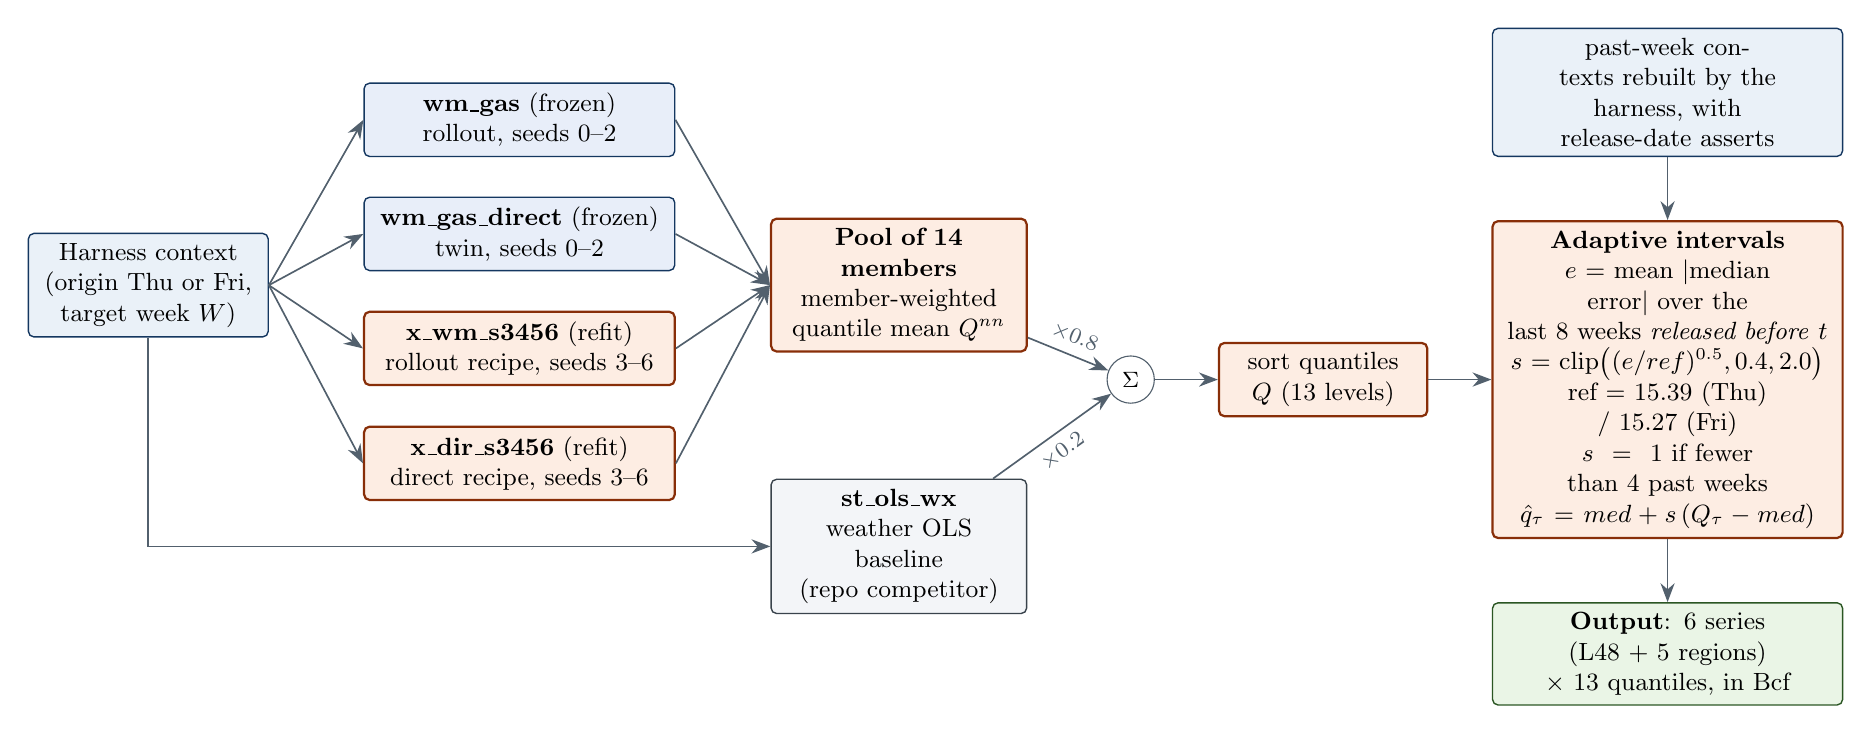
\begin{tikzpicture}[node distance=5mm and 8mm]
\node[data,text width=2.8cm] (ctx) {Harness context\\(origin Thu or Fri,\\target week $W$)};
\node[model,right=12mm of ctx,yshift=21mm,text width=3.7cm] (m1) {\textbf{wm\_gas} (frozen)\\rollout, seeds 0--2};
\node[model,below=of m1,text width=3.7cm] (m2) {\textbf{wm\_gas\_direct} (frozen)\\twin, seeds 0--2};
\node[newb,below=of m2,text width=3.7cm] (m3) {\textbf{x\_wm\_s3456} (refit)\\rollout recipe, seeds 3--6};
\node[newb,below=of m3,text width=3.7cm] (m4) {\textbf{x\_dir\_s3456} (refit)\\direct recipe, seeds 3--6};
\foreach \m in {m1,m2,m3,m4} \draw[arr] (ctx.east)--(\m.west);
\node[newb,right=12mm of m2,yshift=-6.5mm,text width=3.0cm] (pool) {\textbf{Pool of 14 members}\\member-weighted\\quantile mean $Q^{nn}$};
\foreach \m in {m1,m2,m3,m4} \draw[arr] (\m.east)--(pool.west);
\node[greyb,below=16mm of pool,text width=3.0cm] (ols) {\textbf{st\_ols\_wx}\\weather OLS baseline\\(repo competitor)};
\draw[arr] (ctx.south) |- (ols.west);
\node[op,right=10mm of pool,yshift=-12mm] (bl) {$\Sigma$};
\draw[arr] (pool) -- node[lab,above,sloped]{$\times 0.8$} (bl);
\draw[arr] (ols) -- node[lab,below,sloped]{$\times 0.2$} (bl);
\node[newb,right=8mm of bl,text width=2.4cm] (sort) {sort quantiles\\$Q$ (13 levels)};
\draw[arr] (bl)--(sort);
\node[newb,right=8mm of sort,text width=4.2cm] (adp) {\textbf{Adaptive intervals}\\$e$ = mean $|$median error$|$ over the\\last 8 weeks \emph{released before} $t$\\$s=\mathrm{clip}\big((e/\text{ref})^{0.5},0.4,2.0\big)$\\ref = 15.39 (Thu) / 15.27 (Fri)\\$s=1$ if fewer than 4 past weeks\\$\hat q_\tau=\text{med}+s\,(Q_\tau-\text{med})$};
\draw[arr] (sort)--(adp);
\node[data,above=8mm of adp,text width=4.2cm] (past) {past-week contexts rebuilt by the\\harness, with release-date asserts};
\draw[arr] (past)--(adp);
\node[evalb,below=8mm of adp,text width=4.2cm] (out) {\textbf{Output}: 6 series (L48 + 5 regions)\\$\times$ 13 quantiles, in Bcf};
\draw[arr] (adp)--(out);
\end{tikzpicture}
\end{center}
\vspace{1mm}
\noindent\begin{minipage}[t]{0.48\linewidth}\small
\textbf{How it was chosen (DEV, 6 rolling folds 2019-07 to 2025-06).}
\begin{itemize}
\item The pool of rollout and direct seeds plus OLS, with the weight chosen leave-one-fold-out, reached DEV MAE 15.46 vs 16.23 for the frozen recipe with 7 seeds, lower in all 6 folds.
\item Final frozen weight: 0.2 (full-DEV optimum); DEV MAE 15.39 / 15.27.
\item Interval rule, chosen LOFO on DEV: DEV QS 5.970 $\to$ 5.919.
\end{itemize}
\end{minipage}\hfill
\begin{minipage}[t]{0.48\linewidth}\small
\textbf{TEST result (52 weeks, Thursday / Friday).}
\begin{itemize}
\item MAE 10.63 / 10.46\,Bcf (wm\_gas 11.53 / 11.56); QS 4.14 / 4.07 (4.59 / 4.56).
\item Significant vs OLS on MAE and QS; not significant vs wm\_gas.
\item 80\% coverage 0.885 / 0.904; intervals 17\% narrower than with fixed widths.
\item Leak test with the global data store scrambled: 0 of 22 forecasts changed.
\end{itemize}
\end{minipage}
\keyline

% =====================================================================================================================
% PAGE 5  wm_power + blend
% =====================================================================================================================
\newpage
\pagetitle{5. wm\_power: physics-informed merit-order world model (German day-ahead power)}{\texttt{tools/power/wm\_models.py} (\texttt{PhysWM}, \texttt{arch=phys}), wrapper \texttt{tools/power/wm\_power.py}. $d=64$, 14 days of context, auxiliary loss weight 0.3, lr $10^{-3}$ OneCycle, batch 64, 1,500 steps, seeds 0--2. The blend was added by the audit.}

\begin{center}
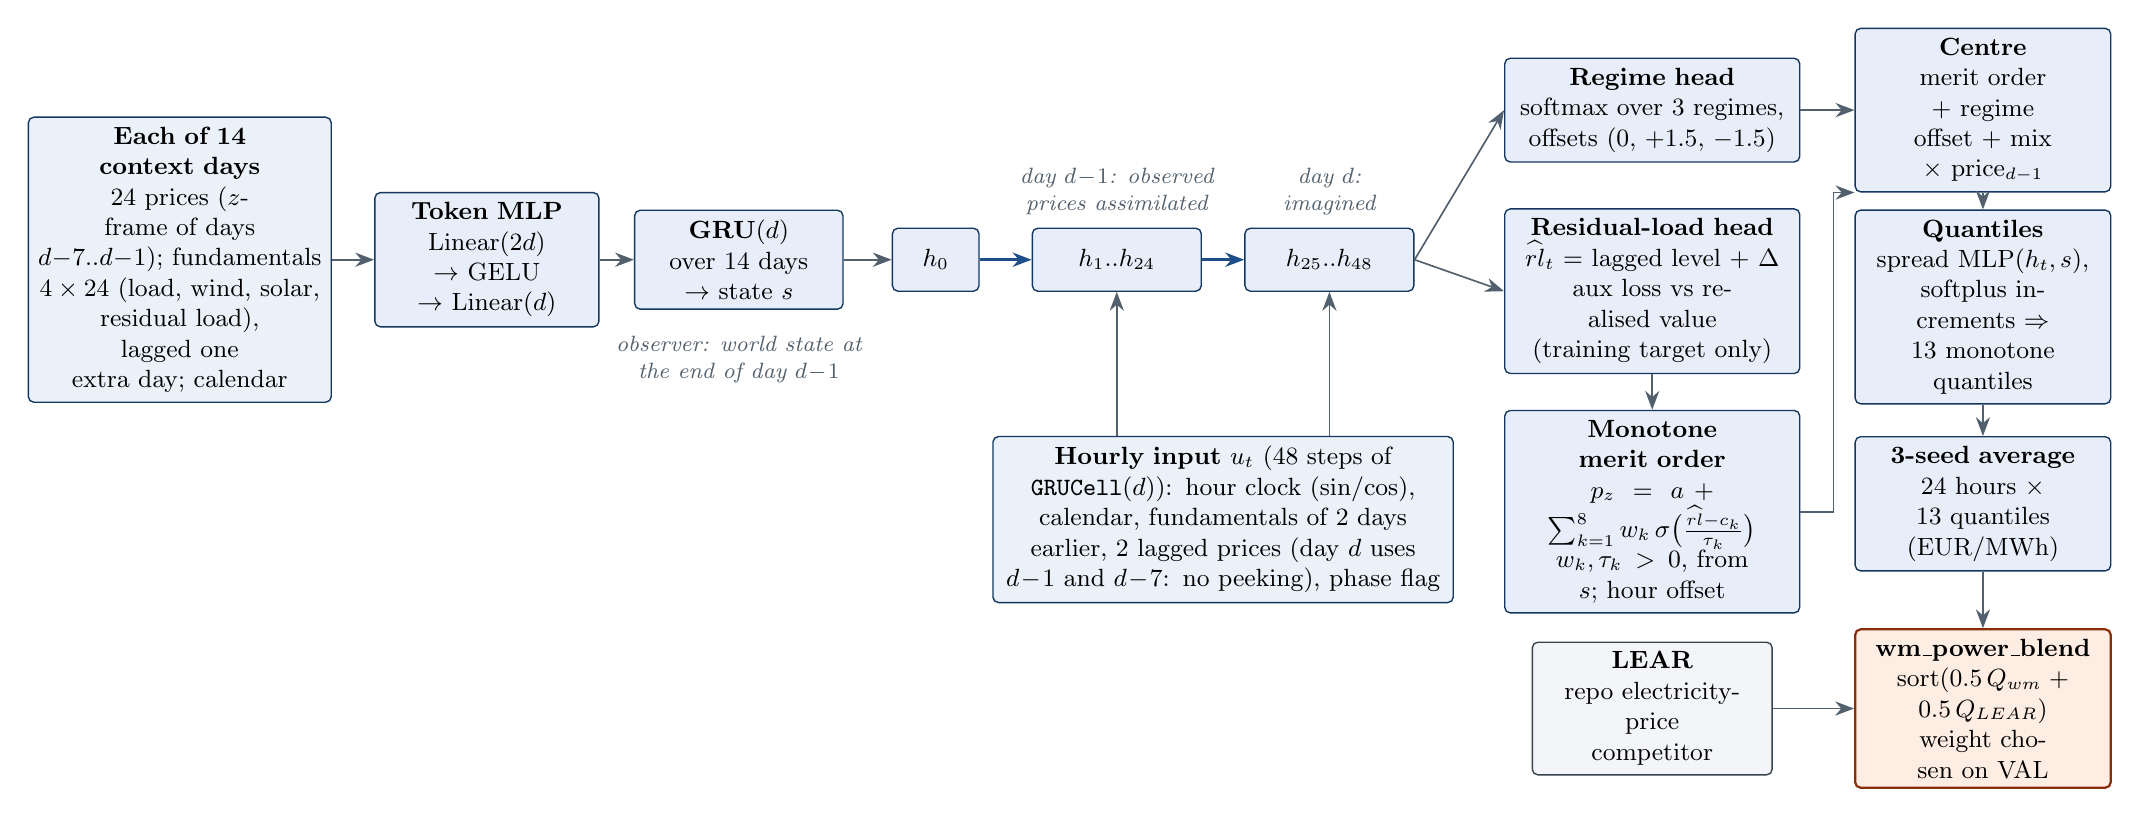
\begin{tikzpicture}[x=1cm,y=1cm]
\node[data,text width=3.6cm] (x) at (2.0,0) {\textbf{Each of 14 context days}\\24 prices ($z$-frame of days\\$d\!-\!7..d\!-\!1$); fundamentals\\$4\times24$ (load, wind, solar,\\residual load), lagged one\\extra day; calendar};
\node[model,text width=2.6cm] (tok) at (5.9,0) {\textbf{Token MLP}\\Linear($2d$) $\to$ GELU\\$\to$ Linear($d$)};
\node[model,text width=2.4cm] (gru) at (9.1,0) {\textbf{GRU}($d$)\\over 14 days\\$\to$ state $s$};
\draw[arr] (x)--(tok); \draw[arr] (tok)--(gru);
\node[lab,anchor=north] at (9.1,-0.85) {observer: world state at\\the end of day $d\!-\!1$};
\node[model,minimum width=1.1cm] (h0) at (11.6,0) {$h_0$};
\node[model,text width=1.9cm] (hA) at (13.9,0) {$h_1 .. h_{24}$};
\node[model,text width=1.9cm] (hB) at (16.6,0) {$h_{25} .. h_{48}$};
\draw[arr] (gru)--(h0); \draw[rarr] (h0)--(hA); \draw[rarr] (hA)--(hB);
\node[lab,anchor=south] at (13.9,0.45) {day $d\!-\!1$: observed\\prices assimilated};
\node[lab,anchor=south] at (16.6,0.45) {day $d$:\\imagined};
\node[data,text width=5.6cm] (uin) at (15.25,-3.3) {\textbf{Hourly input} $u_t$ (48 steps of \texttt{GRUCell}($d$)): hour clock (sin/cos), calendar, fundamentals of 2 days earlier, 2 lagged prices (day $d$ uses $d\!-\!1$ and $d\!-\!7$: no peeking), phase flag};
\draw[arr] (uin.north-|hA) -- (hA.south); \draw[arr] (uin.north-|hB) -- (hB.south);
% heads
\node[model,text width=3.5cm] (reg) at (20.7,1.9) {\textbf{Regime head}\\softmax over 3 regimes,\\offsets $(0,\,+1.5,\,-1.5)$};
\node[model,text width=3.5cm] (rl) at (20.7,-0.4) {\textbf{Residual-load head}\\$\widehat{rl}_t$ = lagged level + $\Delta$\\aux loss vs realised value\\(training target only)};
\node[model,text width=3.5cm] (mo) at (20.7,-3.2) {\textbf{Monotone merit order}\\$p_z = a + \sum_{k=1}^{8} w_k\,\sigma\big(\frac{\widehat{rl}-c_k}{\tau_k}\big)$\\$w_k,\tau_k>0$, from $s$; hour offset};
\draw[arr] (hB.east)--(reg.west); \draw[arr] (hB.east)--(rl.west); \draw[arr] (rl)--(mo);
\node[model,text width=3.0cm] (cen) at (24.9,1.9) {\textbf{Centre}\\merit order + regime\\offset + mix $\times$ price$_{d-1}$};
\draw[arr] (reg)--(cen); \draw[arr] (mo.east) -- (23.0,-3.2) |- (cen.south west);
\node[model,text width=3.0cm] (q) at (24.9,-0.6) {\textbf{Quantiles}\\spread MLP$(h_t, s)$,\\softplus increments $\Rightarrow$\\13 monotone quantiles};
\draw[arr] (cen)--(q);
\node[model,text width=3.0cm] (e3) at (24.9,-3.1) {\textbf{3-seed average}\\24 hours $\times$ 13 quantiles\\(EUR/MWh)};
\draw[arr] (q)--(e3);
\node[newb,text width=3.0cm] (bl) at (24.9,-5.7) {\textbf{wm\_power\_blend}\\sort$(0.5\,Q_{\text{wm}} + 0.5\,Q_{\text{LEAR}})$\\weight chosen on VAL};
\node[greyb,text width=2.8cm] (lear) at (20.7,-5.7) {\textbf{LEAR}\\repo electricity-price\\competitor};
\draw[arr] (e3)--(bl); \draw[arr] (lear)--(bl);
\end{tikzpicture}
\end{center}
\vspace{-2mm}
\noindent{\small\textbf{Twin} (\texttt{wm\_power\_direct}): every hour is one GRUCell step from $s$. \textbf{TEST} (365 days): wm\_power P2 0.747, QS 9.02, cov80 0.752; twin P2 0.739, QS 9.08. \textbf{Blend}: QS 8.60 (significant vs wm\_power and LEAR), P2 0.755 (significant vs LEAR only).}
\keyline

% =====================================================================================================================
% PAGE 6  wm_fin + blend
% =====================================================================================================================
\newpage
\pagetitle{6. wm\_fin: RSSM world model on an intraday clock (crypto realized volatility)}{\texttt{tools/fin/wm\_core.py} (\texttt{RSSM}, ``DreamerV3-lite''), wrapper \texttt{tools/fin/wm\_fin.py}. $d=64$, $z=16$, 4 prior sub-steps (6 h each) per day, window $W=14$ days, weekday-of-$D$ input; lr $2\times10^{-3}$, 800 steps; 3 seeds refit on labels $\leq$ 2025-06-30 (16 training coins). The blend was added by the audit.}

\begin{center}
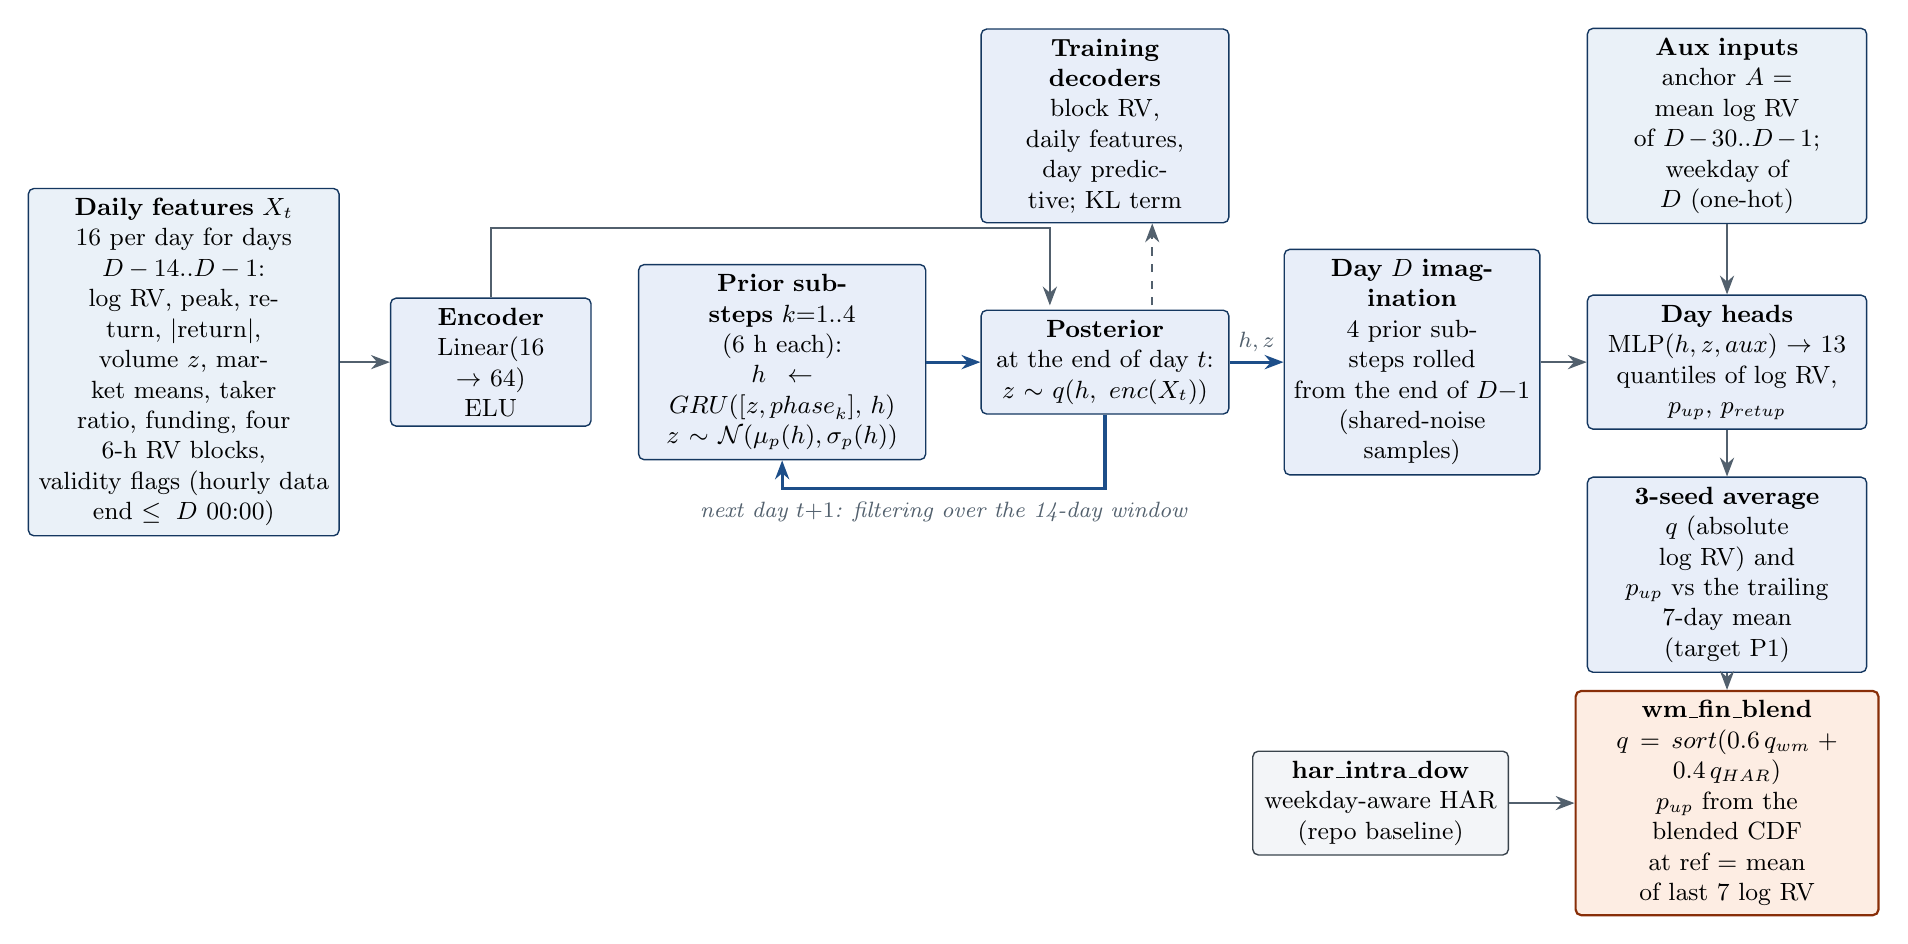
\begin{tikzpicture}[x=1cm,y=1cm]
\node[data,text width=3.7cm] (f) at (2.0,0) {\textbf{Daily features} $X_t$\\16 per day for days $D\!-\!14..D\!-\!1$:\\log RV, peak, return, $|$return$|$,\\volume $z$, market means, taker\\ratio, funding, four 6-h RV blocks,\\validity flags (hourly data\\end $\leq D$ 00:00)};
\node[model,text width=2.3cm] (enc) at (5.9,0) {\textbf{Encoder}\\Linear(16 $\to$ 64)\\ELU};
\draw[arr] (f)--(enc);
\node[model,text width=3.4cm] (prior) at (9.6,0) {\textbf{Prior sub-steps} $k{=}1..4$\\(6 h each):\\$h \leftarrow \text{GRU}([z,\text{phase}_k],\,h)$\\$z \sim \mathcal{N}(\mu_p(h),\sigma_p(h))$};
\node[model,text width=2.9cm] (post) at (13.7,0) {\textbf{Posterior}\\at the end of day $t$:\\$z \sim q(h,\ \text{enc}(X_t))$};
\draw[rarr] (prior)--(post);
\draw[arr] (enc.north) -- (5.9,1.7) -- (13.0,1.7) -- (13.0,0.72);
\draw[rarr] (post.south) -- (13.7,-1.6) -- (9.6,-1.6) -- (prior.south);
\node[lab,anchor=north] at (11.65,-1.65) {next day $t{+}1$: filtering over the 14-day window};
\node[model,text width=2.9cm] (dec) at (13.7,3.0) {\textbf{Training decoders}\\block RV, daily features,\\day predictive; KL term};
\draw[darr] (14.3,0.72) -- (14.3,0.72 |- dec.south);
% day D
\node[model,text width=3.0cm] (roll) at (17.6,0) {\textbf{Day $D$ imagination}\\4 prior sub-steps rolled\\from the end of $D\!-\!1$\\(shared-noise samples)};
\draw[rarr] (post)--node[lab,above]{$h, z$}(roll);
\node[data,text width=3.3cm] (aux) at (21.6,3.0) {\textbf{Aux inputs}\\anchor $A$ = mean log RV\\of $D\!-\!30..D\!-\!1$;\\weekday of $D$ (one-hot)};
\node[model,text width=3.3cm] (head) at (21.6,0) {\textbf{Day heads}\\MLP$(h, z, \text{aux})$ $\to$ 13\\quantiles of log RV,\\$p_{\text{up}}$, $p_{\text{ret up}}$};
\draw[arr] (roll)--(head); \draw[arr] (aux)--(head);
\node[model,text width=3.3cm] (ens) at (21.6,-2.7) {\textbf{3-seed average}\\$q$ (absolute log RV) and\\$p_{\text{up}}$ vs the trailing\\7-day mean (target P1)};
\draw[arr] (head)--(ens);
\node[newb,text width=3.6cm] (bl) at (21.6,-5.6) {\textbf{wm\_fin\_blend}\\$q = \text{sort}(0.6\,q_{\text{wm}} + 0.4\,q_{\text{HAR}})$\\$p_{\text{up}}$ from the blended CDF\\at ref = mean of last 7 log RV};
\node[greyb,text width=3.0cm] (har) at (17.2,-5.6) {\textbf{har\_intra\_dow}\\weekday-aware HAR\\(repo baseline)};
\draw[arr] (ens)--(bl); \draw[arr] (har)--(bl);
\end{tikzpicture}
\end{center}
\vspace{-1mm}
\noindent\begin{minipage}[t]{0.55\linewidth}\small
\textbf{Twin} (\texttt{wm\_direct}): the day heads read the filtered state at the end of $D\!-\!1$, with no day-$D$ rollout (identical modules and losses).\\
\textbf{Other frozen pillars} (not diagrammed): wm\_fin\_cl (continual SGD, 1 step per day), wm\_agent (Dreamer-style actor-critic), PPO/DQN twins.
\end{minipage}\hfill
\begin{minipage}[t]{0.42\linewidth}\small
\textbf{TEST} (24 coins): wm\_fin P1 0.727, QS 0.1471; twin P1 0.724, QS 0.1465; har\_intra\_dow P1 0.731. \textbf{Blend}: P1 0.740, QS 0.1459. Significant vs wm\_fin on P1; not vs har\_intra\_dow.
\end{minipage}
\keyline

% =====================================================================================================================
% PAGE 7  wm_sv oil
% =====================================================================================================================
\newpage
\pagetitle{7. wm\_sv: stochastic-volatility world model (WTI crude oil)}{\texttt{tools/commodity/wm\_models.py} (\texttt{SVWM}), wrapper \texttt{tools/commodity/wm\_commodity.py}. Input: 128 days of WTI only. $d=64$, about 25,191 parameters per member; lr $2\times10^{-3}$ cosine, batch 64, 600 steps; training windows end before 2023-01-01; seeds 0--2, mean of log-level quantiles.}

\begin{center}
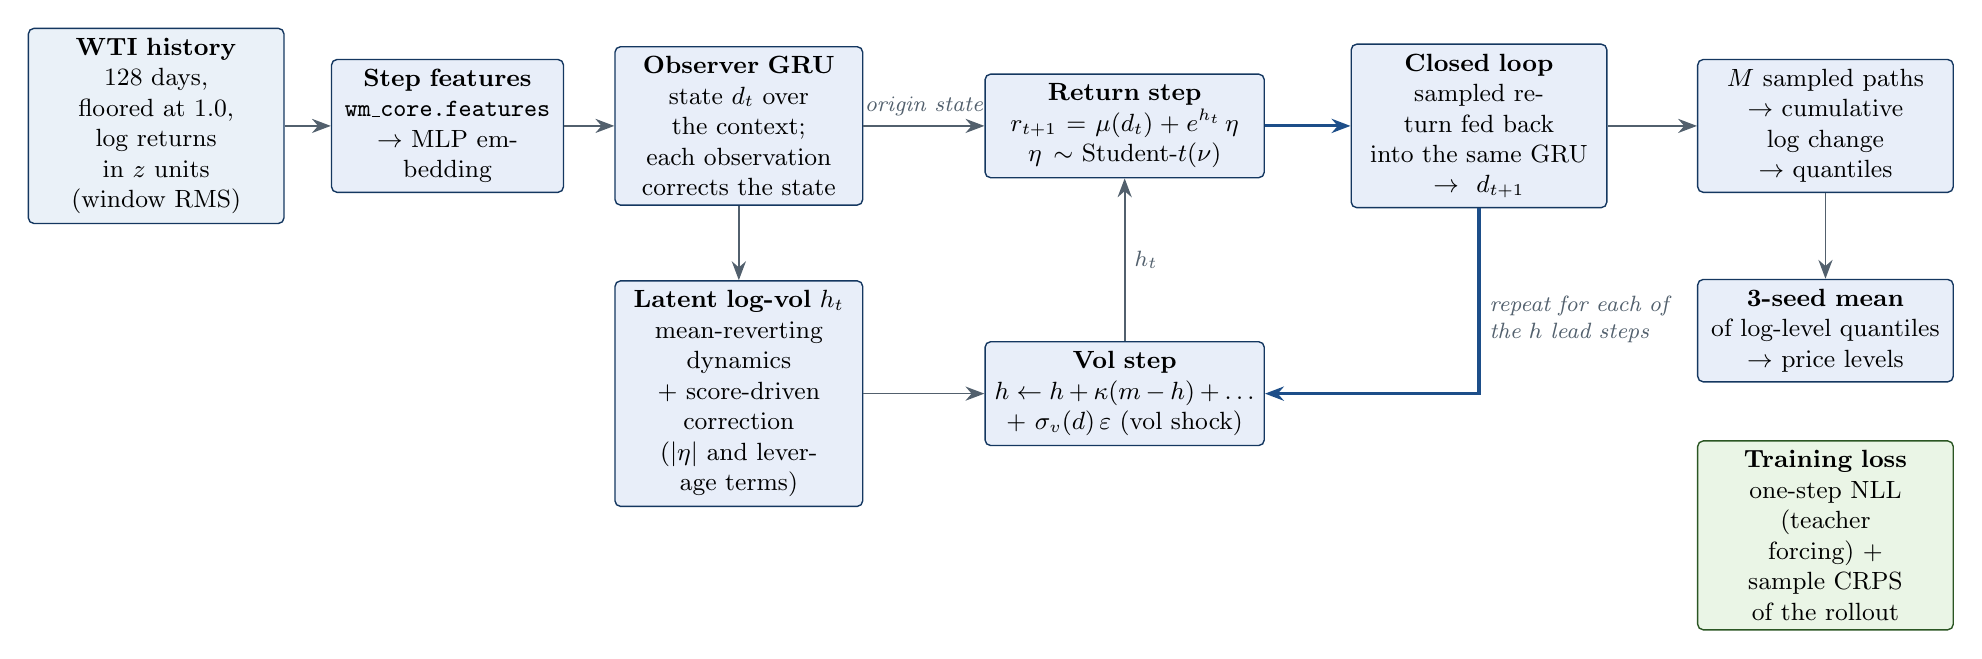
\begin{tikzpicture}[x=1cm,y=1cm]
\node[data,text width=3.0cm] (x) at (2.0,0) {\textbf{WTI history}\\128 days, floored at 1.0,\\log returns in $z$ units\\(window RMS)};
\node[model,text width=2.7cm] (emb) at (5.7,0) {\textbf{Step features}\\\texttt{wm\_core.features}\\$\to$ MLP embedding};
\node[model,text width=2.9cm] (obs) at (9.4,0) {\textbf{Observer GRU}\\state $d_t$ over the context;\\each observation\\corrects the state};
\node[model,text width=2.9cm] (hv) at (9.4,-3.4) {\textbf{Latent log-vol} $h_t$\\mean-reverting dynamics\\+ score-driven correction\\($|\eta|$ and leverage terms)};
\draw[arr] (x)--(emb); \draw[arr] (emb)--(obs); \draw[arr] (obs)--(hv);
\node[model,text width=3.3cm] (ret) at (14.3,0) {\textbf{Return step}\\$r_{t+1} = \mu(d_t) + e^{h_t}\,\eta$\\$\eta \sim$ Student-$t(\nu)$};
\node[model,text width=3.3cm] (vol) at (14.3,-3.4) {\textbf{Vol step}\\$h \leftarrow h + \kappa(m-h) + \dots$\\$+\ \sigma_v(d)\,\varepsilon$ (vol shock)};
\draw[arr] (obs)--node[lab,above]{origin state}(ret); \draw[arr] (hv)--(vol); \draw[arr] (vol)--node[lab,right]{$h_t$}(ret);
\node[model,text width=3.0cm] (fb) at (18.8,0) {\textbf{Closed loop}\\sampled return fed back\\into the same GRU\\$\to d_{t+1}$};
\draw[rarr] (ret)--(fb);
\draw[rarr] (fb.south) |- node[lab,pos=0.3,right,text width=2.3cm,align=left]{repeat for each of the $h$ lead steps} (vol.east);
\node[model,text width=3.0cm] (paths) at (23.2,0) {$M$ sampled paths\\$\to$ cumulative log change\\$\to$ quantiles};
\draw[arr] (fb)--(paths);
\node[model,text width=3.0cm] (ens) at (23.2,-2.6) {\textbf{3-seed mean}\\of log-level quantiles\\$\to$ price levels};
\draw[arr] (paths)--(ens);
\node[evalb,text width=3.0cm] (loss) at (23.2,-5.2) {\textbf{Training loss}\\one-step NLL (teacher\\forcing) + sample CRPS\\of the rollout};
\end{tikzpicture}
\end{center}
\vspace{1mm}
\noindent{\small\textbf{Twin} (\texttt{wm\_sv\_direct}): lead $k$ is one step from the origin state, $d_k=\mathrm{GRU}(\text{emb}_k, d_{\text{origin}})$, decoded as a Student-$t$ with scale $e^{h_{\text{origin}}+m(d_k)}\sqrt{k}$; nothing is sampled step by step.\\
\textbf{TEST} ($h=1$, 246 origins): QS 0.01052 vs random walk 0.01056 (skill +0.45\%, $p=0.479$, a tie); twin 0.01056. No improvement model was built, because the signal is indistinguishable from a random walk.}
\keyline

% =====================================================================================================================
% PAGE 8  forward test
% =====================================================================================================================
\newpage
\pagetitle{8. Forward-test architecture (frozen 1 November 2026, 17:47 UTC)}{\texttt{tools/forward/forward\_eval.py}, \texttt{tools/forward/FREEZE.json}. Scores the frozen models only on data published after they were frozen.}

\begin{center}
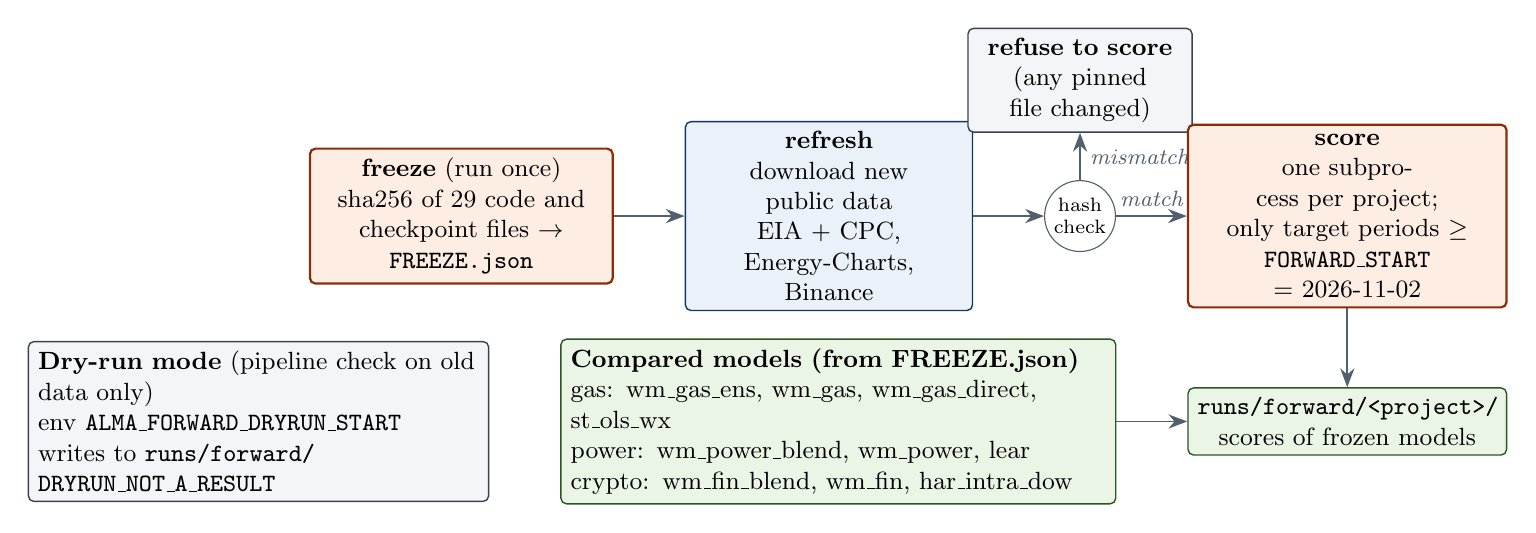
\begin{tikzpicture}[node distance=6mm and 9mm]
\node[newb,text width=3.6cm] (fz) {\textbf{freeze} (run once)\\sha256 of 29 code and\\checkpoint files $\to$\\\texttt{FREEZE.json}};
\node[data,right=of fz,text width=3.4cm] (rf) {\textbf{refresh}\\download new public data\\EIA + CPC, Energy-Charts,\\Binance};
\node[op,right=of rf,minimum size=9mm,font=\scriptsize,align=center] (chk) {hash\\check};
\node[greyb,above=6mm of chk,text width=2.6cm] (stop) {\textbf{refuse to score}\\(any pinned file changed)};
\draw[arr] (fz)--(rf); \draw[arr] (rf)--(chk); \draw[arr] (chk)--node[lab,right]{mismatch}(stop);
\node[newb,right=of chk,text width=3.8cm] (sc) {\textbf{score}\\one subprocess per project;\\only target periods $\geq$\\\texttt{FORWARD\_START} = 2026-11-02};
\draw[arr] (chk)--node[lab,above]{match}(sc);
\node[evalb,below=10mm of sc,text width=3.8cm] (res) {\texttt{runs/forward/<project>/}\\scores of frozen models};
\draw[arr] (sc)--(res);
\node[evalb,left=of res,text width=6.8cm,align=left] (mods) {\textbf{Compared models (from FREEZE.json)}\\gas: wm\_gas\_ens, wm\_gas, wm\_gas\_direct, st\_ols\_wx\\power: wm\_power\_blend, wm\_power, lear\\crypto: wm\_fin\_blend, wm\_fin, har\_intra\_dow};
\draw[arr] (mods)--(res);
\node[greyb,left=of mods,text width=5.6cm,align=left] (dry) {\textbf{Dry-run mode} (pipeline check on old data only)\\env \texttt{ALMA\_FORWARD\_DRYRUN\_START}\\writes to \texttt{runs/forward/}\\\texttt{DRYRUN\_NOT\_A\_RESULT}};
\end{tikzpicture}
\end{center}
\vspace{3mm}
\noindent{\small\textbf{Data arrival}: first EIA storage report 2026-11-05; gas release \#20 on 2027-03-18 and \#52 on 2027-10-28; power and crypto day 60 on 2026-12-31 and day 365 on 2027-11-01. These follow the publication calendars, with holiday shifts possible.}
\keyline

\end{document}
